\documentclass[12pt]{beamer}

\setbeamerfont{block body alerted}{size=\small}

\usetheme{Madrid}
\useoutertheme{shadow}

\usepackage{amsfonts}
\usepackage{hyperref}
\usepackage[super,comma,numbers]{natbib}
\renewcommand{\bibnumfmt}[1]{[#1]}
\bibliographystyle{apsrev4-1}

\title[Annealed model]{An annealed model of diffusion in semi-permeable domains}
\author[Hathcock group]{A. Brown | Hathcock group}
\date{January 16, 2026}


\newcommand{\abs}[1]{\left| #1 \right|} % | |
\newcommand{\norm}[1]{\left|\left| #1 \right|\right|} % || ||
\newcommand{\bra}[1]{\left\langle #1 \right|} % < |
\newcommand{\ket}[1]{\left| #1 \right\rangle} % | >
\newcommand{\braket}[2]{\left\langle #1 \middle| #2 \right\rangle} % < | >
\newcommand{\ketbra}[2]{\left| #1 \right\rangle \left\langle #2 \right|} % | >< |
\newcommand{\mbraket}[3]{\left\langle #1 \middle| #2 \middle| #3 \right\rangle} % < | | >


\begin{document}

\maketitle

\begin{frame}{Reading progress}
    \begin{itemize}
        \item \textit{Conformal Field Theory} (CFT) - Chpt.~5
        \begin{itemize}
            \item Goal: Complete reading Chpt.~1-7, 10, 12, 13-15 before end of term
        \end{itemize}
        \item \textit{Critical Dynamics} (CD) - Chpt.~4
        \begin{itemize}
            \item Goal: Complete reading Chpt.~1-9 before end of term
        \end{itemize}
        \item \textit{Quantum Field Theory and the Standard Model} (QFT) - Chpt.~18
        \begin{itemize}
            \item Goal: Complete reading Chpt.~14-23 before end of term
        \end{itemize}
        \item \textit{Field Theory of Non-Equilibrium Systems} (FTNE) - DNS
        \begin{itemize}
            \item Goal: Complete reading Chpt.~1-2, 6, 9-12 before end of term
        \end{itemize}
        \item Working on finishing typesetting for CFT Chpt.~4 \& CD Chpt.~3
    \end{itemize}
\end{frame}

\begin{frame}{The model}
    \begin{itemize}
        \item The particle begins at the centre of a sphere $\mathcal{B}_1 \subset \mathbb{R}^n$ of radius $r_1$ with diffusivity $D_1$, and membrane permissivity $\kappa_1$
        \pause
        \item Reflected Brownian motion (RBM) occurs, governed by the Skorokhod equation~\cite{PhysRevLett.125.078102}
        \begin{equation} \label{eq:skorokhod}
            d X_t^{(1)} = \sqrt{2 D_1} \, d W_t + n(x) \, d \ell_t^{(1)},
        \end{equation}
        until the boundary local time,
        \begin{equation} \label{eq:boundary-local-time}
            \ell_t^{(1)} := 2 D n \int_{\partial \mathcal{B}_1} d^{n-1} x \, \int_0^t \delta (X_s - x) \, d s
        \end{equation}
        exceeds a random variable $\hat{\ell}^{(1)}$, 
        whose probability law obeys $\mathbb{P} \{ \hat{\ell}^{(1)} > \ell \} = e^{- q_1 \ell}$, for $q_1 = \kappa_1 / D_1$
    \end{itemize}
\end{frame}

\begin{frame}{The model}
    \begin{itemize}
        \item Once the (boundary) \emph{reaction time} $\mathcal{T}_1 = \inf{\left\{ t > 0 : \ell_t^{(1)} > \hat{\ell}^{(1)} \right\}}$ for the domain has been reached,
        an new RBM initiates at the centre of another sphere $\mathcal{B}_2$ with sampled parameters $(D_2, r_2, \kappa_2)$
        \item The same occurs once the analogously defined reaction time, $\mathcal{T}_2$, for the second sphere has been reached, and so on
    \end{itemize}
    \pause
    \begin{figure}
        \centering
        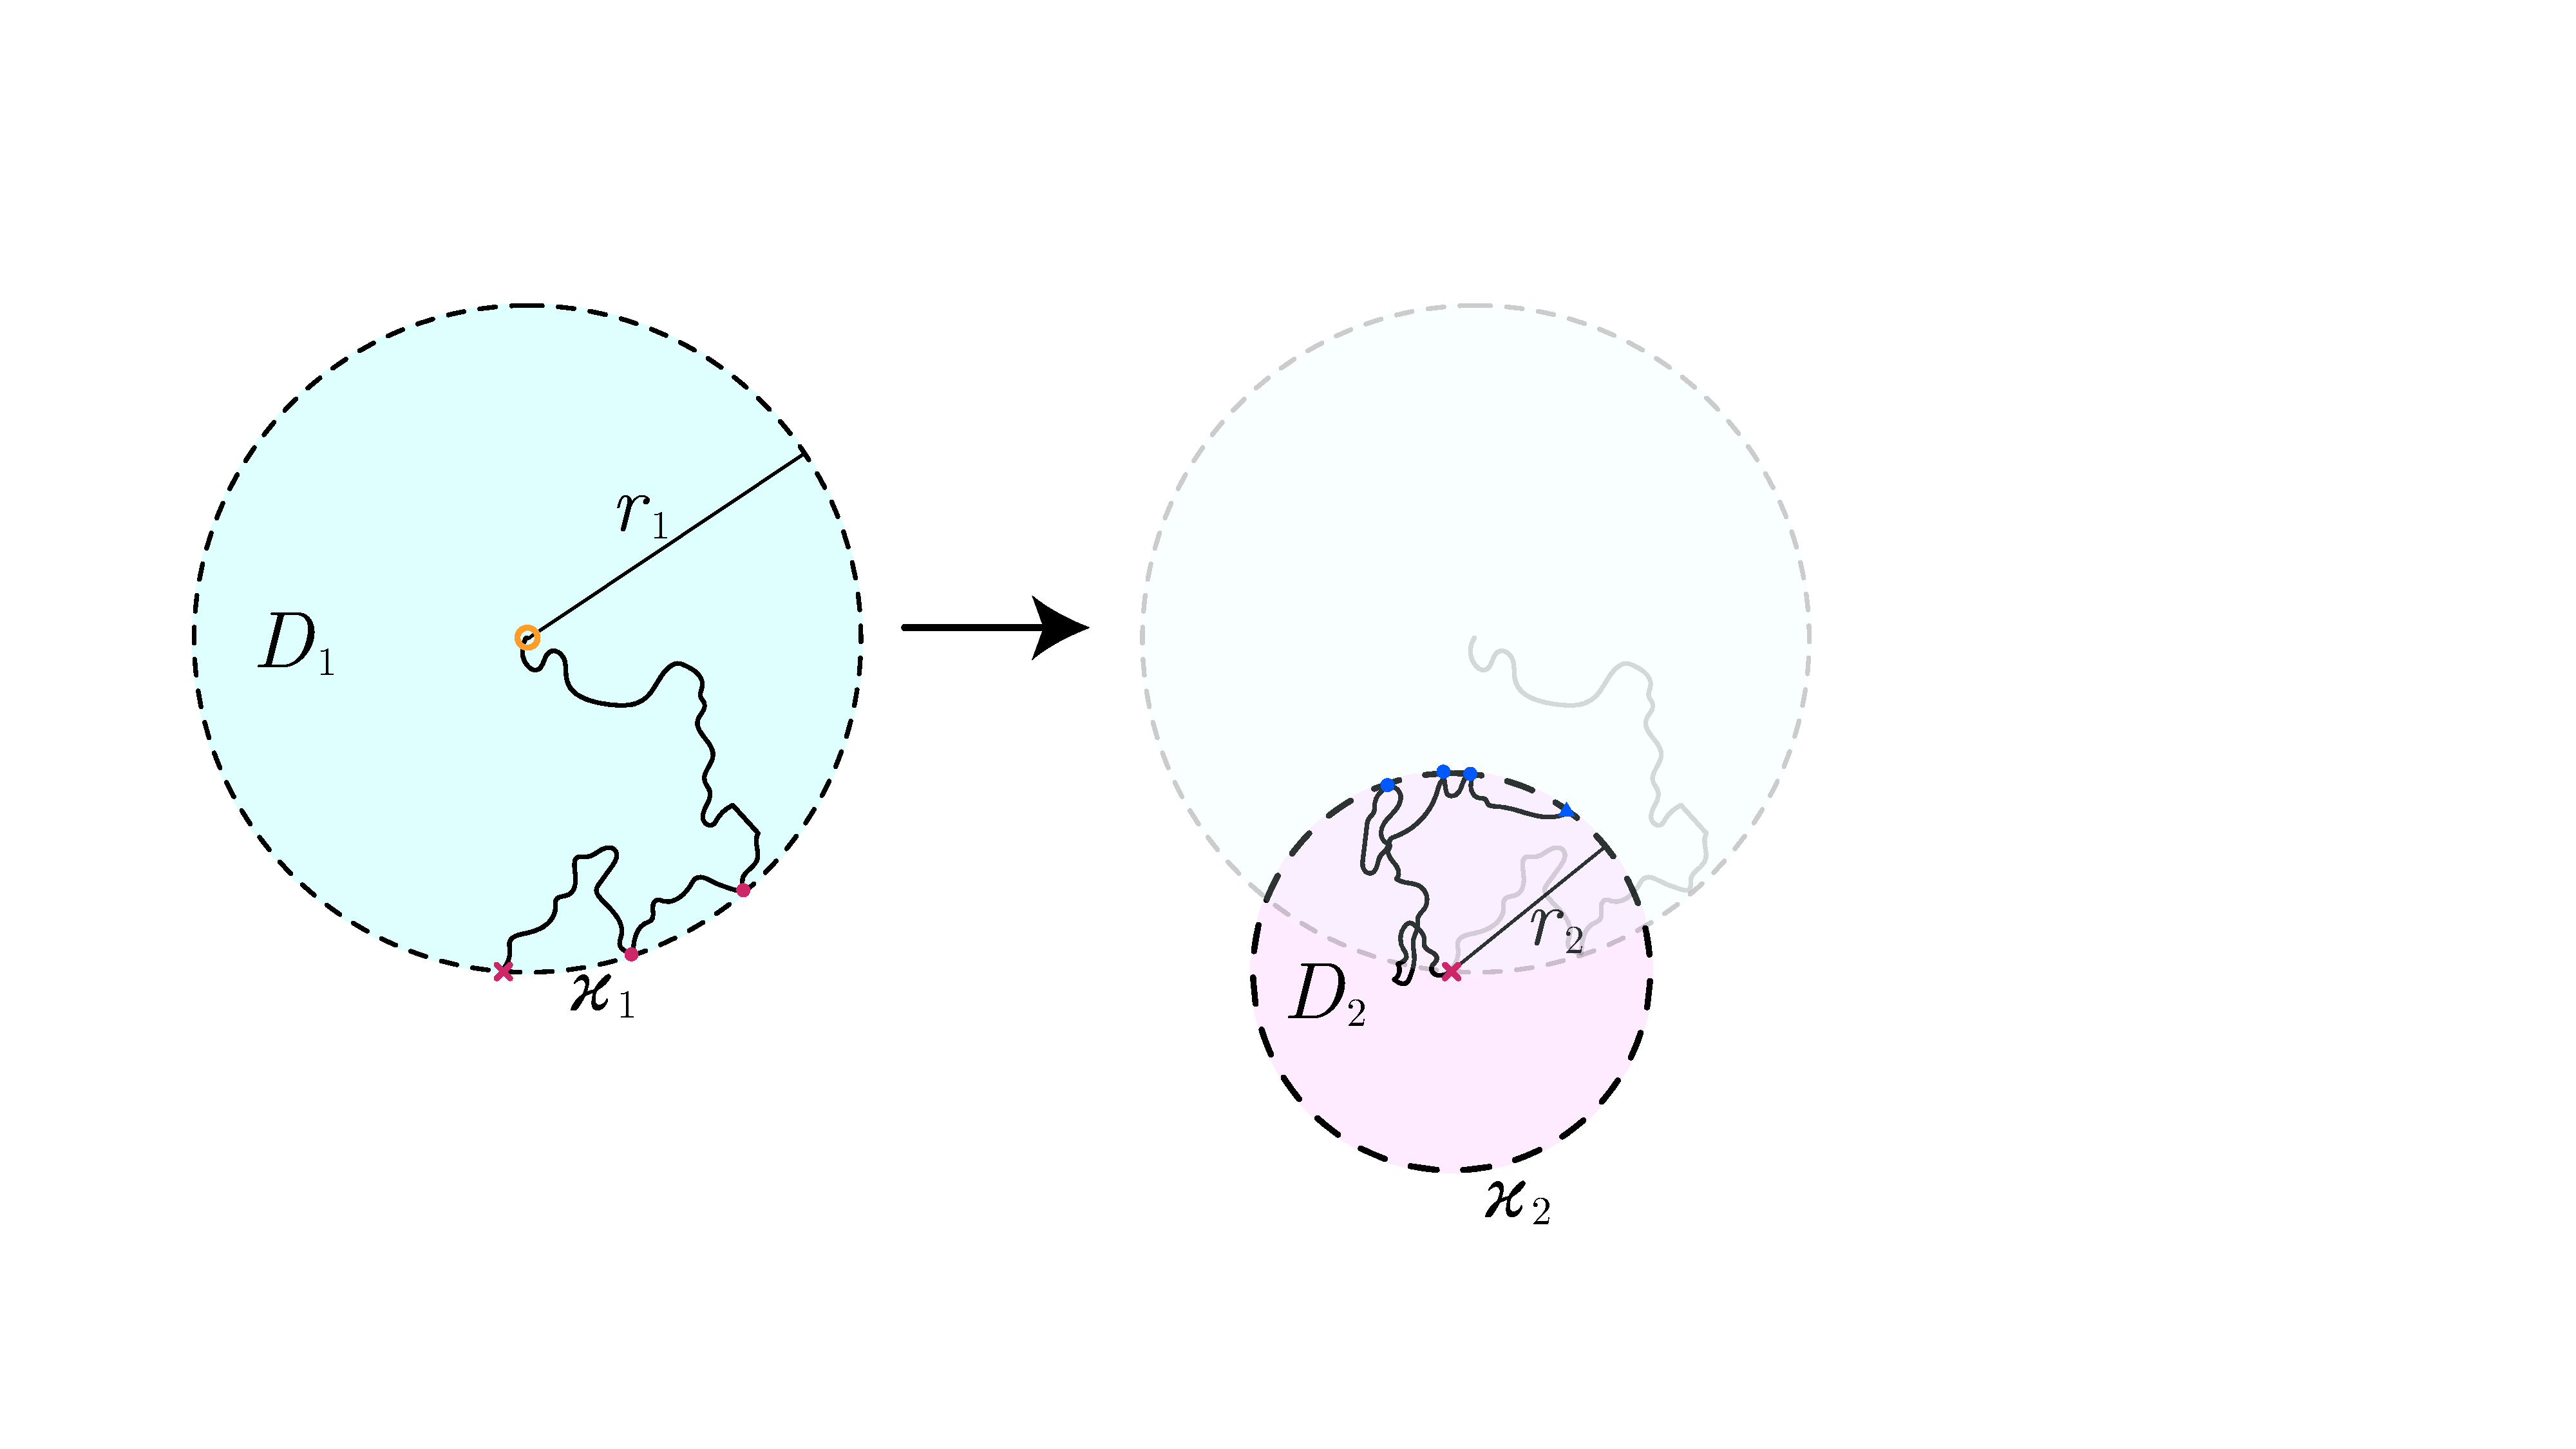
\includegraphics[width=0.65\textwidth]{figures/annealed-model.pdf}
    \end{figure}
\end{frame}

\begin{frame}{The exit time density}
    \begin{itemize}
        \item Coarse graining: view the exit from a domain as a single step on a (continuous) ``lattice''.
        Assume that direction of step is unbiased (symmetry of sphere)~\cite{PhysRevLett.112.150603}
        \pause
        \item Let $U (\ell, t \mid x_0)$ denote the PDF of the first time $\mathcal{T}_\ell$ 
        when the boundary local time exceeds a fixed value $\ell$, conditioned on $x_0$
        {%
            \setlength{\belowdisplayskip}{0pt}
            \setlength{\belowdisplayshortskip}{0pt}
            \begin{equation}
                \mathcal{T}_\ell = \inf{\left\{ t > 0 : \ell_t > \ell \right\}}
            \end{equation}
        }%
        \pause
        \item $\mathbb{P}_{x_0} \{ \ell_t > \ell \} \iff \mathbb{P}_{x_0} \{ t > \mathcal{T}_\ell \}$ and so
        \begin{equation}
            U (\ell, t \mid x_0) = \frac{\partial \mathbb{P}_{x_0} \{ t > \mathcal{T}_\ell \}}{\partial t}
            = \int_{\ell}^\infty d \ell' \, \frac{\partial \rho (\ell', t \mid x_0)}{\partial t},
        \end{equation}
        where $\rho$ is the PDF of the boundary local time~\cite{PhysRevLett.125.078102}
    \end{itemize}
\end{frame}

\begin{frame}{The exit time density}
    \begin{itemize}
        \item After taking a temporal Laplace transform ($t \xrightarrow[]{\mathcal{L}} \alpha$), 
        it can be shown that $U$ permits a spectral representation in terms of the eigenfunctions of the Dirichlet-to-Neumann (DtN) operator~\cite{PhysRevLett.125.078102},
        {%
            \setlength{\belowdisplayskip}{0pt}
            \setlength{\belowdisplayshortskip}{0pt}
            \begin{equation}
                \Tilde{U} (\ell, \alpha \mid x_0) = \sum_n e^{- \mu_n^\alpha \ell} [V_n^{(\alpha)} (x_0)]^* \int_{\partial \Omega} d^{n-1} s \, V_n^{(\alpha)} (s)
            \end{equation}
        }%
        \pause
        \begin{itemize}
            \item Let $w$ be a solution to the Helmholtz equation $(\alpha - D \Delta) w = 0$ with Dirichlet BC $w |_{\partial \Omega} = f$.
            The DtN operator $\mathcal{M}_\alpha$ is defined by $[\mathcal{M}_\alpha f] (x) = \partial_n w |_{x \in \partial \Omega}$
        \end{itemize}
    \end{itemize}
\end{frame}

\begin{frame}{Spectral representation}
    \begin{itemize}
        \item In general we can write the eigenequation as
        \begin{equation}
            \mathcal{M}_\alpha v_n^{(\alpha)} (x) = \mu_n^{(\alpha)} v_n^{(\alpha)} (x)
        \end{equation}
        \item The nature of the solution depends explicitly on the dimension.
        Choose the disk $\Omega = \{ \abs{x} < R, x \in \mathbb{R}^2 \}$
        \pause
        \item We allow for arbitrary boundary data $f (\theta)$. 
        Let $u(r, \phi) = Q_n (r) e^{i n \phi}$ with $\lambda = \sqrt{\alpha / D}$.
        The modified Helmholtz equation reads
        {
            \setlength{\belowdisplayskip}{0pt}
            \setlength{\belowdisplayshortskip}{0pt}
            \begin{equation}
                r^2 Q_n'' (r) + r Q_n' (r) - \left( n^2 + \lambda^2 r^2 \right) Q_n (r) = 0
            \end{equation}
        }
        \pause
        \item Solutions are modified Bessel functions.
        Enforcing regularity,
        \begin{equation}
            u (r, \phi, \alpha) = \sum_{n = -\infty}^\infty a_n I_{\abs{n}} (\lambda r) e^{i n \phi}
        \end{equation}
    \end{itemize}
\end{frame}

\begin{frame}{Spectral representation}
    \begin{itemize}
        \item But now we note that $e^{i n \phi}$ is not altered by the normal derivative.
        As such, we may identify the eigenfunctions $v_n (\phi) = e^{i n \phi}$ as the Fourier modes and compute
        \begin{equation}
            [\mathcal{M}_\alpha v_n] (\phi) = \partial_r u_n (R, \phi) = \lambda \frac{I_{\abs{n}}'(\lambda R)}{I_{\abs{n}}(\lambda R)} e^{i n \phi},
        \end{equation}
        so we can identify the eigenvalues
        \begin{equation}
            \mu_n^{(\alpha)} = \lambda \frac{I_{\abs{n}}' (\lambda R)}{I_{\abs{n}} (\lambda R)} = \lambda \frac{d}{dz} \log{I_{\abs{n}} (\lambda R)}, \qquad
            \lambda = \sqrt{\alpha/D}
        \end{equation}
        \pause
        \item We can approximate these eigenvalues at long times, $\lambda R \ll 1$ as
        \begin{equation}
            \mu_n^{(\alpha)} \sim \frac{n}{R} + \frac{\lambda^2 R}{2 (n+1)} - \frac{\lambda^4 R^3}{8 (n+1)^2 (n+2)} + \mathcal{O}(\lambda R^5)
        \end{equation}
    \end{itemize}
\end{frame}

\begin{frame}{References}
    \bibliography{references}
\end{frame}




\begin{frame}{Details of spectral representation}
    Probabilistically, we can understand diffusion within a domain $\Omega$ with semi-permeable boundary of permissivity $\kappa (x)$ as the BVP~\cite{JChemPhys.1.5115030}
    \begin{subequations}
        \begin{align} \label{eq:diffusion-equation}
            \frac{\partial G (x, t \mid x_0)}{\partial t} - D \Delta G (x, t, \mid x_0) & = 0, \quad x \in \Omega \\ \label{eq:initial-condition}
            G (x, t=0 \mid x_0) & = \delta (x - x_0) \\ \label{eq:robin-boundary}
            \left( D \frac{\partial}{\partial n_x} + \kappa (x) \right) G (x, t \mid x_0) & = 0, \quad x \in \partial \Omega.
        \end{align}
    \end{subequations}
    If we are to take the Laplace transform with respect to time, 
    \begin{equation} \label{eq:laplace-transform}
        \Tilde{G} (x, \alpha \mid x_0) = \int_0^\infty e^{- \alpha t} G (x, t \mid x_0) \, dt,
    \end{equation}
    this reduces Eq.~\eqref{eq:diffusion-equation} to the inhomogeneous Helmholtz problem:
    \begin{equation} \label{eq:modified-helmholtz}
        (\alpha - D \Delta) \Tilde{G} (x, \alpha \mid x_0) = \delta (x - x_0).
    \end{equation}
\end{frame}

\begin{frame}{Details of spectral representation}
    Since the problem is linear, we are free to take
    \begin{equation} \label{eq:propagator-split}
        \Tilde{G} (x, \alpha \mid x_0) = \Tilde{G}_0 (x, \alpha \mid x_0) + \Tilde{g} (x, \alpha \mid x_0),
    \end{equation}
    where $\Tilde{G}_\infty$ is the propagator with absorbing boundary conditions,
    \begin{subequations}
        \begin{align} \label{eq:dirichlet-propagator}
            (\alpha - D \Delta) \Tilde{G}_\infty (x, \alpha \mid x_0) & = \delta (x - x_0), \quad x \in \Omega \\ \label{eq:absorbing-bc}
            \Tilde{G}_\infty (x, \alpha \mid x_0) & = 0, \quad x \in \partial \Omega.
        \end{align}
    \end{subequations}
    Thus the unknown contribution which reacts with the boundary satisfies
    \begin{subequations}
        \begin{align} \label{eq:non-absorbed-propagator}
            (\alpha - D \Delta) \Tilde{g} (x, \alpha \mid x_0) & = 0, \quad x \in \Omega \\ \label{eq:non-absorbed-bc}
            \left( D \frac{\partial}{\partial n_x} + \kappa (x) \right) \Tilde{g} (x, \alpha \mid x_0) & = \Tilde{j}_\infty (x, \alpha \mid x_0), \quad x \in \partial \Omega,
        \end{align}
    \end{subequations}
    where $\Tilde{j}_0$ is the Laplace transform of the diffusive flux density at time $t$ on a point of the perfectly reactive surface.
\end{frame}

\begin{frame}{Details of spectral representation}
    Consider the Dirichlet BVP
    \begin{subequations}
        \begin{align} \label{eq:helmholtz}
            (\alpha - D \Delta) u (x, \alpha) & = 0, \quad x \in \Omega \\ \label{eq:dirichlet-bc}
            u (x, \alpha) & = f (x, \alpha), \quad x \in \partial \Omega.
        \end{align}
    \end{subequations}
    We define the Dirichlet-to-Neumann (DtN) $\mathcal{M}_\alpha$ as
    \begin{equation} \label{eq:dtn-operator}
        [\mathcal{M}_\alpha f] (x) = \left( \frac{\partial u}{\partial n} \right)_{x \in \partial \Omega},
    \end{equation}
    which determines the flux produced at the boundary by $u$ (Neumann BC) given boundary value $f$.
    To this end, on the boundary, we may write the boundary conditions for the unknown contribution to the propagator Eq.~\eqref{eq:non-absorbed-propagator} as 
    (with $\mathcal{Q} = \kappa (y) / D$)
    \begin{equation} \label{eq:non-absorbed-bc-operator}
        \left( \mathcal{M}_\alpha + \mathcal{Q} \right) \Tilde{g} (y, \alpha \mid x_0) = \frac{1}{D} \Tilde{j}_\infty (y, \alpha \mid x_0), \quad y \in \partial \Omega.
    \end{equation}
\end{frame}

\begin{frame}{Details of spectral representation}
    Formally, we may invert Eq.~\eqref{eq:non-absorbed-bc-operator},
    \begin{equation}
        \Tilde{g} (y, \alpha \mid x_0) = \left( \mathcal{M}_\alpha + \mathcal{Q} \right)^{-1} \frac{\Tilde{j}_\infty (y, \alpha \mid x_0)}{D}.
    \end{equation}
    This is now the form of a Dirichlet problem, allowing us to write the bulk solution
    \begin{equation}
        \Tilde{g} (x, \alpha \mid x_0) = \int_{\partial \Omega} d^{n-1} y \, \Tilde{j}_\infty (y, \alpha \mid x) \Tilde{g} (y, \alpha \mid x_0), \quad x \in \Omega.
    \end{equation}
    If we let the surface propagation operator be written $\mathcal{O} = \left( \mathcal{M}_\alpha + \mathcal{Q} \right)^{-1}$,
    \begin{equation}
        \Tilde{G} (x, \alpha \mid x_0) = \Tilde{G}_\infty (x, \alpha \mid x_0) + 
        \int_{\partial \Omega} d^{n-1} y \, \Tilde{j}_\infty (y, \alpha \mid x) \frac{\mathcal{O}}{D} \Tilde{j}_\infty (y, \alpha \mid x_0).
    \end{equation}
\end{frame}

\begin{frame}{Details of spectral representation}
    The identity $\Tilde{j}_\infty (y, \alpha \mid y_0) = \delta (y - y_0)$ for $y, y_0 \in \partial \Omega$ implies that the propagator between two surface points
    \begin{equation} \label{eq:surface-dlt-relation}
        D (\mathcal{M}_\alpha + \mathcal{Q}) \Tilde{G} (y, \alpha \mid y_0) = \delta (y - y_0).
    \end{equation}
    Now we may express the bulk propagator as
    \begin{multline} \label{eq:propagator-expansion}
        \Tilde{G} (x, \alpha \mid x_0) = \Tilde{G}_\infty (x, \alpha \mid x_0) + \\
        \int_{\partial \Omega} d y_1 \, d y_2 \, 
        \Tilde{j}_\infty (y_2, \alpha \mid x) \frac{\Tilde{G} (y_2, \alpha \mid y_1)}{D} \Tilde{j}_\infty (y_1, \alpha \mid x_0).
    \end{multline} 
    In braket notation, eigenvalues of the DtN operator satisfy the eigenequation
    \begin{equation}
        \mathcal{M}_\alpha \ket{v_n^{\alpha} (x)} = \mu_n^{\alpha} \ket{v_n^{\alpha} (x)}.
    \end{equation}
\end{frame}

\begin{frame}{Details of spectral representation}
    Provided $\partial \Omega$ is bounded, the eigenvalues are non-negative and the eigenfunctions form a complete, orthonormal basis on the boundary.
    We may hence resolve the identity and insert it into Eq.~\eqref{eq:propagator-expansion}:
    \begin{multline}
        \Tilde{G} (x, \alpha \mid x_0) = \Tilde{G}_\infty (x, \alpha \mid x_0) \\
        + \frac{1}{D} \sum_{n, m} \int_{\partial \Omega} d y_1 \, d y_2 \, \Tilde{j}_\infty \ket{v_n^{(\alpha)} (s)} \mbraket{v_n^{(\alpha)} (s)}{\mathcal{O}}{v_m^{(\alpha)} (s')} \bra{v_m^{(\alpha)} (s')} \Tilde{j}_\infty
    \end{multline}
    If the permissivity is taken to be constant, the matrix is diagonal
    \begin{equation}
        \mbraket{v_n^{(\alpha)} (s)}{(\mathcal{M}_\alpha + q)^{-1}}{v_m^{(\alpha)} (s')} = \left( \mu_n^{(\alpha)} + q \right)^{-1} \delta_{n,m}.
    \end{equation}
\end{frame}

\begin{frame}{Details of the spectral representation}
    Inserting the element into the propagator,
    \begin{multline}
        \Tilde{G} (x, \alpha \mid x_0) = \Tilde{G}_\infty (x, \alpha \mid x_0)
        + \frac{1}{D} \sum_n \frac{[V_n^{(\alpha)} (x_0)]^* V_n^{(\alpha)} (x)}{\mu_n^{(\alpha)} + q},
    \end{multline}
    where we have defined the projections
    \begin{equation}
        V_n^{(\alpha)} (x) = \int_{\partial \Omega} d^{n-1} y \, v_n^{(\alpha)} (y) \Tilde{j}_\infty (y, \alpha \mid x).
    \end{equation}
\end{frame}

\begin{frame}{Bessel ratio asymptotic form}
    We begin with the standard power series
    \begin{align*}
        I_n (z) & = \sum_{k=0}^\infty \frac{1}{k! \Gamma (n + k + 1)} \left( \frac{z}{2} \right)^{n + 2k} \\
        & = \frac{1}{n!} \left( \frac{z}{2}^n \right)^n \left[ 1 + \frac{z^2}{4 (n+1)} + \frac{z^4}{32 (n+1) (n+2)} + \mathcal{O} (z^6) \right].
    \end{align*}
    Taking the logarithm, performing an expansion $\log{(1 + x)} \sim x - \frac{x^2}{2} + \frac{x^3}{3} + \mathcal{O} (x^4)$, and differentiating,
    \begin{equation}
        \frac{I_n' (z)}{I_n (z)} = \frac{n}{z} + \frac{z}{2 (n+1)} - \frac{z^3}{8 (n+1)^2 (n+2)} + \mathcal{O}(z^5)
    \end{equation}
\end{frame}

\end{document}